\paragraph{QuizziPedia::Front-End::Views::ResultsQuestionnaireView}
\begin{figure} [ht]
	\centering
	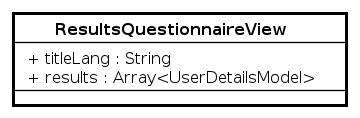
\includegraphics[scale=0.80]{UML/Classi/Front-End/QuizziPedia_Front-end_ResultsQuestionnarieView.png}
	\caption{QuizziPedia::Front-End::Views:ResultsQuestionnaireView}
\end{figure} \FloatBarrier
\begin{itemize}
	\item \textbf{Descrizione}: \textit{view\ped{G}} contenente i risultati conseguiti dagli utenti che hanno compilato il proprio questionario;
	\item \textbf{Utilizzo}: permette di visualizzare i risultati di ogni utente conseguiti nella compilazione del questionario;
	\item \textbf{Relazioni con altre classi}:
	\begin{itemize}
		\item \textbf{IN \texttt{ResultsQuestionnaireModelView}}: classe di tipo modelview la cui istanziazione è contenuta all'interno della variabile di ambiente \texttt{\$scope} di \textit{Angular\ped{G}}. All'interno di essa sono presenti le variabili e i metodi necessari per il \textit{Two-Way Data-Binding\ped{G}} tra la \text{view\ped{G}} \texttt{ResultsQuestionnaireView} e il \textit{controller\ped{G}} \texttt{ResultsController}; 
		\item \textbf{IN \texttt{LangModel}}: rappresenta il modello delle informazioni per la giusta traduzione dell'applicazione.
	\end{itemize}
	\item \textbf{Attributi}:
	\begin{itemize}
		\item \texttt{+ results: Array<UserDetailsModel>} \\ \texttt{array} contenente un oggetto per ogni iscritto che ha compilato il questionario. L'oggetto sarà composto dai campi: \texttt{nome} e \texttt{cognome} e \texttt{valutazione};
		\item \texttt{+ titleLang: String} \\ Attributo che viene utilizzato per visualizzare la giusta traduzione del titolo della pagina, in italiano o in inglese.
	\end{itemize}
\end{itemize}